% =============================================================================
\section{The Basic Shapes}\label{sec:shapes}
All objects are built from the fifteen \emph{unit} meshes listed in \Cref{tab:shapes}. Each mesh is
centred at the origin and has a size of about one unit, so a part of any size is obtained by scaling it.
The meshes are generated once at start-up (\texttt{gfx/Shapes.cpp}) and stay on the GPU; every part of
every object is only a reference to one of these meshes plus a $4\times4$ matrix. The pictures show each
mesh with the edges of its triangles drawn on top.

\paragraph{Generation rules.} Flat shapes are written as lists of corner points. Every face has its own
vertices, so that the face has one flat normal and the edges stay sharp; a quad face $(a,b,c,d)$ is split
into the triangles $(a,b,c)$ and $(a,c,d)$. Round shapes are generated by loops over angles. For a ring of
$n$ steps the angle is $\theta_i = 2\pi i/n$, and the side of a cylinder with bottom radius $r_b$ and top
radius $r_t$ uses
\[
\mathbf{p}_i^{top} = (r_t\cos\theta_i,\ 0.5,\ r_t\sin\theta_i),\quad
\mathbf{p}_i^{bot} = (r_b\cos\theta_i,\ -0.5,\ r_b\sin\theta_i),\quad
\mathbf{n}_i = \operatorname{normalize}(\cos\theta_i,\ r_b-r_t,\ \sin\theta_i).
\]
Neighbouring ring points form one side quad
$(\mathbf{p}_i^{bot},\ \mathbf{p}_{i+1}^{bot},\ \mathbf{p}_{i+1}^{top},\ \mathbf{p}_i^{top})$,
and a cap is a fan of triangles around the centre vertex $(0,\pm0.5,0)$. Round shapes have one normal per
vertex pointing straight out of the surface, so they look smooth even with few sides.

{\small
\setlength{\tabcolsep}{4pt}
\begin{longtable}{@{}c P{2.1cm} P{8.2cm} r@{}}
\caption{The basic shapes, how their vertices are generated, and their vertex / triangle counts}\label{tab:shapes}\\
\toprule
Shape & Name & Vertices & V / T \\ \midrule
\endfirsthead
\toprule
Shape & Name & Vertices & V / T \\ \midrule
\endhead
\bottomrule
\endfoot
\raisebox{-0.8\height}{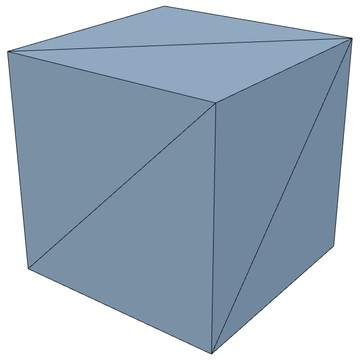
\includegraphics[width=2.1cm]{shape_0}} & Cube & 8 corners $(\pm.5,\pm.5,\pm.5)$ (\Cref{fig:cube}); each of the 6 faces has its own 4 vertices and the face normal & \svCube\ / \stCube \\
\raisebox{-0.8\height}{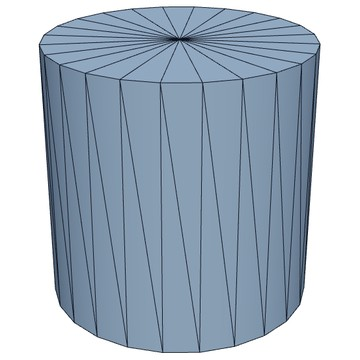
\includegraphics[width=2.1cm]{shape_1}} & Cylinder & ring loop with $r_b=r_t=0.5$, $n=24$, two caps & \svCylinder\ / \stCylinder \\
\raisebox{-0.8\height}{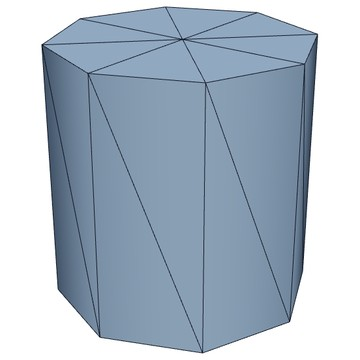
\includegraphics[width=2.1cm]{shape_2}} & Cylinder (low) & the same with $n=8$; used for tree trunks and bamboo & \svCylinderLow\ / \stCylinderLow \\
\raisebox{-0.8\height}{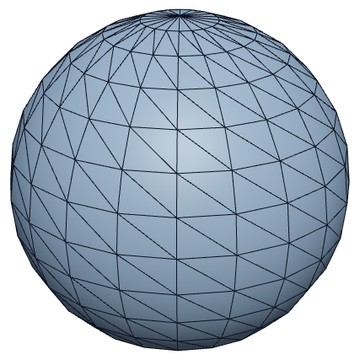
\includegraphics[width=2.1cm]{shape_3}} & Sphere & $\mathbf{p}_{ij}=0.5(\sin\phi_i\cos\theta_j,\ \cos\phi_i,\ \sin\phi_i\sin\theta_j)$, $\phi_i=\pi i/14$, $\theta_j=2\pi j/20$, normal $\mathbf{n}=2\mathbf{p}$ & \svSphere\ / \stSphere \\
\raisebox{-0.8\height}{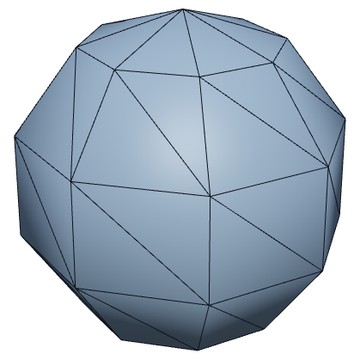
\includegraphics[width=2.1cm]{shape_4}} & Sphere (low) & the same with 5 rings and 8 sectors; foliage blobs, rocks & \svSphereLow\ / \stSphereLow \\
\raisebox{-0.8\height}{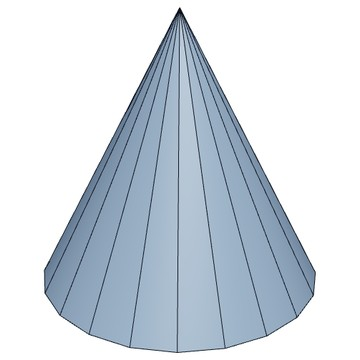
\includegraphics[width=2.1cm]{shape_5}} & Cone & ring loop with $r_t=0$ (all top vertices meet at the tip $(0,0.5,0)$), $n=20$, bottom cap & \svCone\ / \stCone \\
\raisebox{-0.8\height}{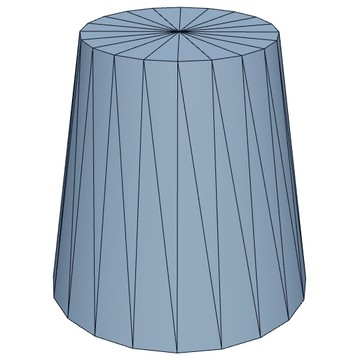
\includegraphics[width=2.1cm]{shape_6}} & Truncated cone & ring loop with $r_t=0.35$, $n=20$, two caps; cups, pots, limbs & \svTruncatedCone\ / \stTruncatedCone \\
\raisebox{-0.8\height}{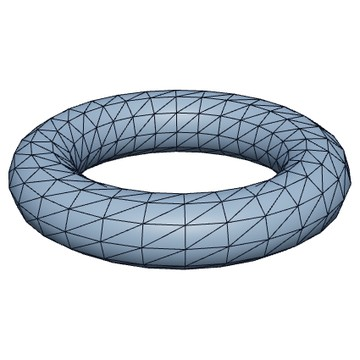
\includegraphics[width=2.1cm]{shape_7}} & Torus & $\mathbf{p}(u,w)=(0.4+0.1\cos w)(\cos u,0,\sin u)+(0,0.1\sin w,0)$, $28\times10$ steps & \svTorus\ / \stTorus \\
\raisebox{-0.8\height}{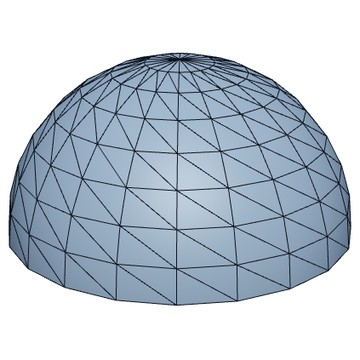
\includegraphics[width=2.1cm]{shape_8}} & Hemisphere & sphere formula with $\phi\in[0,\pi/2]$ (8 rings) plus a flat disc at $y=0$ & \svHemisphere\ / \stHemisphere \\
\raisebox{-0.8\height}{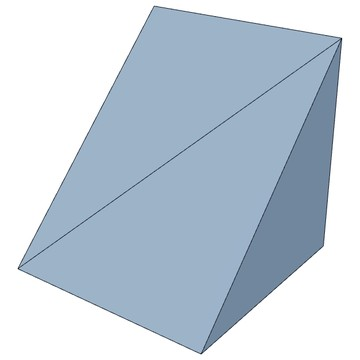
\includegraphics[width=2.1cm]{shape_9}} & Wedge & left side $w_0(-.5,-.5,.5)$, $w_1(-.5,-.5,-.5)$, $w_2(-.5,.5,-.5)$; right side $w_3,w_4,w_5$ = the same with $x=+.5$; 2 triangles and 3 quads & \svWedge\ / \stWedge \\
\raisebox{-0.8\height}{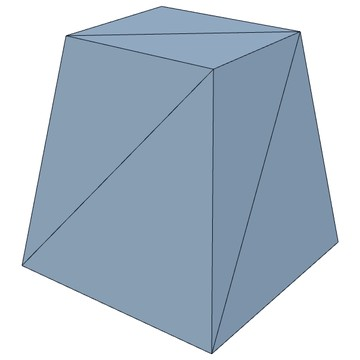
\includegraphics[width=2.1cm]{shape_10}} & Tapered box & bottom corners $(\pm.5,-.5,\pm.5)$, top corners $(\pm.35,.5,\pm.3)$; side normal $\mathbf{n}=\operatorname{normalize}((\mathbf{b}-\mathbf{a})\times(\mathbf{d}-\mathbf{a}))$ & \svTaperedBox\ / \stTaperedBox \\
\raisebox{-0.8\height}{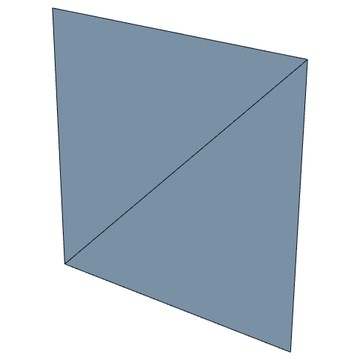
\includegraphics[width=2.1cm]{shape_11}} & Quad & $(-.5,-.5,0)$, $(.5,-.5,0)$, $(.5,.5,0)$, $(-.5,.5,0)$, normal $(0,0,1)$; fronds, vines & \svQuad\ / \stQuad \\
\raisebox{-0.8\height}{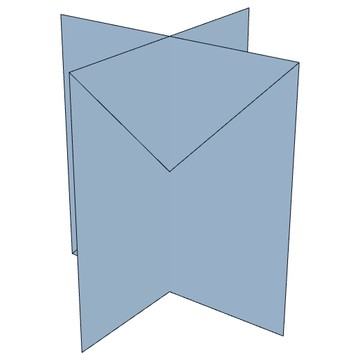
\includegraphics[width=2.1cm]{shape_12}} & Cross card & two crossed quads with $y\in[0,1]$ (base on the ground); grass, ferns, flowers & \svCrossCard\ / \stCrossCard \\
\raisebox{-0.8\height}{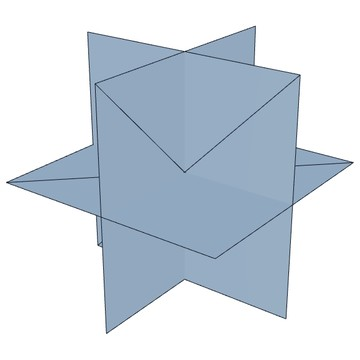
\includegraphics[width=2.1cm]{shape_13}} & Leaf card & three quads through the centre, one in each plane ($xy$, $yz$, $xz$); leaf clusters & \svLeafCard\ / \stLeafCard \\
\raisebox{-0.8\height}{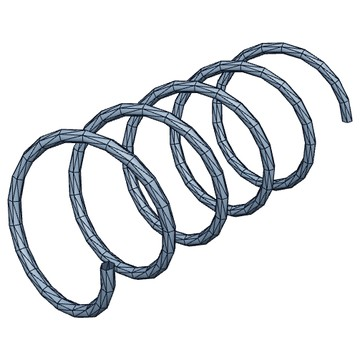
\includegraphics[width=2.1cm]{shape_14}} & Coil & a 6-sided ring around each of 101 points of the helix $\mathbf{c}(t)=(R\cos 2\pi kt,\ R\sin 2\pi kt,\ L(t-0.5))$, $k=5$ turns & \svCoil\ / \stCoil \\
\end{longtable}}

\begin{figure}[H]
\centering
\begin{minipage}{0.40\linewidth}
\centering
\begin{tikzpicture}[scale=2.1,font=\scriptsize]
\coordinate (v0) at (0,0); \coordinate (v1) at (1,0); \coordinate (v2) at (1,1); \coordinate (v3) at (0,1);
\coordinate (v4) at (0.45,-0.35); \coordinate (v5) at (1.45,-0.35); \coordinate (v6) at (1.45,0.65); \coordinate (v7) at (0.45,0.65);
\draw[dashed,gray] (v0)--(v1) (v0)--(v3) (v0)--(v4);
\draw[thick] (v1)--(v2)--(v3) (v4)--(v5)--(v6)--(v7)--cycle (v1)--(v5) (v2)--(v6) (v3)--(v7);
\fill[blue!8,opacity=0.6] (v4)--(v5)--(v6)--(v7)--cycle;
\draw[blue!60] (v4)--(v6);
\foreach \i/\p in {0/left,1/right,2/right,3/left,4/below left,5/below right,6/above right,7/above left} \fill (v\i) circle (0.025) node[\p] {$v_\i$};
\draw[arr,red] (1.9,-0.2)--(2.3,-0.2) node[right]{$x$};
\draw[arr,green!50!black] (1.9,-0.2)--(1.9,0.2) node[above]{$y$};
\draw[arr,blue] (1.9,-0.2)--(1.7,-0.45) node[below]{$z$};
\end{tikzpicture}
\end{minipage}\hfill
\begin{minipage}{0.56\linewidth}
\centering\small
\begin{tabular}{@{}cc|cc@{}}
\toprule
Corner & $(x,y,z)$ & Corner & $(x,y,z)$ \\ \midrule
$v_0$ & $(-.5,-.5,-.5)$ & $v_4$ & $(-.5,-.5,\ .5)$ \\
$v_1$ & $(\ .5,-.5,-.5)$ & $v_5$ & $(\ .5,-.5,\ .5)$ \\
$v_2$ & $(\ .5,\ .5,-.5)$ & $v_6$ & $(\ .5,\ .5,\ .5)$ \\
$v_3$ & $(-.5,\ .5,-.5)$ & $v_7$ & $(-.5,\ .5,\ .5)$ \\
\bottomrule
\end{tabular}

\vspace{0.5em}
Faces: front $(v_4v_5v_6v_7)$, back $(v_1v_0v_3v_2)$, top $(v_7v_6v_2v_3)$,
bottom $(v_0v_1v_5v_4)$, right $(v_5v_1v_2v_6)$, left $(v_0v_4v_7v_3)$.
The front face is split into $(v_4v_5v_6)$ and $(v_4v_6v_7)$.
\end{minipage}
\caption{The unit cube: 8 corners, 6 faces, 12 triangles. The front face (shaded) looks towards $+z$.}\label{fig:cube}
\end{figure}

The ground is one more generated mesh: a $150\times150$ grid whose vertices are lifted to the terrain
height $h(x,z)$ (\Cref{sec:terrain}).

% =============================================================================
\section{Transformations and Hierarchical Modelling}\label{sec:transform}
\subsection{Homogeneous coordinates and the basic transformations}
A point is written as $\mathbf{p}=(x,y,z,1)^T$, so that translation, rotation and scaling are all
$4\times4$ matrix products. The matrices are stored column-major and sent to OpenGL unchanged.
\[
T(\mathbf{t})=\begin{bmatrix}1&0&0&t_x\\0&1&0&t_y\\0&0&1&t_z\\0&0&0&1\end{bmatrix}\qquad
S(\mathbf{s})=\begin{bmatrix}s_x&0&0&0\\0&s_y&0&0\\0&0&s_z&0\\0&0&0&1\end{bmatrix}
\]
\[
R_x(\theta)=\begin{bmatrix}1&0&0&0\\0&\cos\theta&-\sin\theta&0\\0&\sin\theta&\cos\theta&0\\0&0&0&1\end{bmatrix}\quad
R_y(\theta)=\begin{bmatrix}\cos\theta&0&\sin\theta&0\\0&1&0&0\\-\sin\theta&0&\cos\theta&0\\0&0&0&1\end{bmatrix}\quad
R_z(\theta)=\begin{bmatrix}\cos\theta&-\sin\theta&0&0\\\sin\theta&\cos\theta&0&0\\0&0&1&0\\0&0&0&1\end{bmatrix}
\]
A rotation given in degrees $(\theta_x,\theta_y,\theta_z)$ is applied as $R=R_y(\theta_y)\,R_x(\theta_x)\,R_z(\theta_z)$.
Rotation about an arbitrary unit axis $\mathbf{a}$ uses Rodrigues' formula
\[
R(\mathbf{a},\theta) = \cos\theta\,I + (1-\cos\theta)\,\mathbf{a}\mathbf{a}^T + \sin\theta\,[\mathbf{a}]_\times,\qquad
[\mathbf{a}]_\times=\begin{bmatrix}0&-a_z&a_y\\a_z&0&-a_x\\-a_y&a_x&0\end{bmatrix}.
\]
A negative scale factor mirrors a part (used for the fruit bowl and for mirrored book rows).

\subsection{Composite transformation of a part}
Every part of every object is placed with
\[
M_{part} = M_{parent}\cdot T(\text{position})\cdot R(\text{rotation})\cdot S(\text{size}),\qquad
\mathbf{p}_{world} = M_{part}\,\mathbf{p}_{unit}.
\]
Read from right to left, the unit shape is first \textbf{scaled} to its size, then \textbf{rotated}, then
\textbf{translated} to its place inside the parent, and finally carried into the world by the parent's
matrix. The order matters: scaling after a rotation would shear the shape. Normals are transformed with
the normal matrix
\[
N = \big(M_{3\times3}^{-1}\big)^T,\qquad \mathbf{n}_{world} = \operatorname{normalize}(N\,\mathbf{n}),
\]
which keeps them perpendicular to the surface even when a shape is stretched unevenly.

\subsection{Hierarchical modelling with nodes}
Objects are written as trees of \texttt{Node}s. A node stores the matrix of its coordinate frame; a child
node is created with an extra translation and rotation relative to its parent, so moving or turning a
parent moves all of its children:
\begin{lstlisting}
struct Node {
    DrawSink* sink;  Mat4 M;                          // M = this node's world matrix
    Node at(const Vec3& p, const Vec3& rotDeg) const  // child: M * T(p) * R(rot)
        { return Node(*sink, rotateYXZ(translate(M, p), rotDeg)); }
    void part(MeshId mesh, Vec3 pos, Vec3 size, const Material& m, Vec3 rotDeg = {}) const
        { sink->add(mesh, scale(rotateYXZ(translate(M, pos), rotDeg), size), m); }
};
// a sofa arm: a box and a cylinder lying along z (rotated 90 degrees about x)
n.box({x, 0.42f, 0.0f}, {0.16f, 0.44f, 0.88f}, fabric);
n.part(M_CYLINDER, {x, 0.64f, 0.0f}, {0.19f, 0.88f, 0.19f}, fabric, {90, 0, 0});
\end{lstlisting}
The same object code can send its shapes to different \emph{sinks}: the static world, the per-frame list,
a counter, or a collector that records every part with its name (used for the exploded views and part
tables in \Cref{sec:objects}).

\paragraph{A matrix built from corner points.} Some parts are not rectangles (car windows, door glass).
For a parallelogram with corners $\mathbf{a}$, $\mathbf{b}$, $\mathbf{d}$ and $\mathbf{b}+\mathbf{d}-\mathbf{a}$
the model matrix is built directly from the edge vectors:
\[
M = \begin{bmatrix} \mathbf{b}-\mathbf{a} & \mathbf{d}-\mathbf{a} & t\,\hat{\mathbf{n}} & \mathbf{a}+\tfrac12(\mathbf{b}-\mathbf{a})+\tfrac12(\mathbf{d}-\mathbf{a}) \\ 0&0&0&1\end{bmatrix},
\qquad \hat{\mathbf{n}}=\frac{(\mathbf{b}-\mathbf{a})\times(\mathbf{d}-\mathbf{a})}{|(\mathbf{b}-\mathbf{a})\times(\mathbf{d}-\mathbf{a})|},
\]
where $t$ is the thickness. The unit cube corner $(-.5,-.5,0)$ lands exactly on $\mathbf{a}$, $(.5,-.5,0)$
on $\mathbf{b}$ and $(-.5,.5,0)$ on $\mathbf{d}$. A triangle is made the same way from the wedge.
A \emph{beam} between two points $\mathbf{a}$ and $\mathbf{b}$ (pillars, branches) turns the shape's $y$ axis
onto $\mathbf{d}=\mathbf{b}-\mathbf{a}$ with the axis $\mathbf{y}\times\hat{\mathbf{d}}$ and the angle
$\operatorname{atan2}(|\mathbf{y}\times\hat{\mathbf{d}}|,\ \mathbf{y}\cdot\hat{\mathbf{d}})$, and scales it to
the length $|\mathbf{d}|$.

\subsection{Viewing and projection}
The camera matrix is built with \texttt{lookAt} from the eye $\mathbf{e}$, the target $\mathbf{c}$ and the up
vector $\mathbf{u}$:
\[
\mathbf{f}=\frac{\mathbf{c}-\mathbf{e}}{|\mathbf{c}-\mathbf{e}|},\quad
\mathbf{s}=\frac{\mathbf{f}\times\mathbf{u}}{|\mathbf{f}\times\mathbf{u}|},\quad
\mathbf{u}'=\mathbf{s}\times\mathbf{f},\qquad
V=\begin{bmatrix} s_x&s_y&s_z&-\mathbf{s}\cdot\mathbf{e}\\ u'_x&u'_y&u'_z&-\mathbf{u}'\cdot\mathbf{e}\\ -f_x&-f_y&-f_z&\mathbf{f}\cdot\mathbf{e}\\0&0&0&1\end{bmatrix}.
\]
The main view uses a perspective projection with vertical field of view $f$, aspect ratio $a$ and the
near and far planes $z_n$, $z_f$. The sun's shadow camera and the 2D text overlay use orthographic
projections:
\[
P_{persp} = \begin{bmatrix}\frac{1}{a\tan(f/2)}&0&0&0\\0&\frac{1}{\tan(f/2)}&0&0\\0&0&-\frac{z_f+z_n}{z_f-z_n}&-\frac{2z_fz_n}{z_f-z_n}\\0&0&-1&0\end{bmatrix}
\qquad
P_{ortho} = \begin{bmatrix}\frac{2}{r-l}&0&0&-\frac{r+l}{r-l}\\0&\frac{2}{t-b}&0&-\frac{t+b}{t-b}\\0&0&\frac{-2}{z_f-z_n}&-\frac{z_f+z_n}{z_f-z_n}\\0&0&0&1\end{bmatrix}.
\]
A vertex therefore goes through $\mathbf{p}_{clip}=P\,V\,M\,\mathbf{p}$, the perspective division
$\mathbf{p}_{ndc}=\mathbf{p}_{clip}/w_{clip}$, and the viewport transformation to pixels,
\[
x_{win} = \tfrac{W}{2}\,(x_{ndc}+1),\qquad y_{win}=\tfrac{H}{2}\,(y_{ndc}+1),\qquad z_{win}=\tfrac12(z_{ndc}+1).
\]
The field of view $f$ is changed with the mouse wheel between $25^\circ$ and $110^\circ$ (\Cref{sec:camera}),
and the aspect ratio $a=W/H$ follows the window size when the window is resized.
